\section{Introduktion}

\begin{frame}{Introduktion}
	\begin{itemize}
		\onslide<1->{\item Data fra IGISOL ved Jyväskylä Universitet i Finland}
		\onslide<2->{\item Eksperimentet er foretaget i 2020}
		\onslide<3->{\item Undersøgelse af \li og \isotope[12]{B}}
		\onslide<4->{\item \li er god indikator for effektiviteten af setup}
		\onslide<5->{\item \li henfalder ved \be-henfald til \ber, som spontant henfalder ved \al-henfald til to \al-kerner}
	\end{itemize}
\end{frame}


\begin{frame}{\be-henfald}
	\begin{columns}
		\column[]{0.6\textwidth}
		To typer:
		\begin{align*}
		\onslide<2->{&\beta^+:\quad p\rightarrow n + e^+ + \nu_e\\}
		\onslide<2->{&\beta^-:\quad n\rightarrow p + e^- + \bar{\nu_e}}
		\end{align*}
		\onslide<3->{Forskellige Q-værdier:}
		\begin{align*}
		\onslide<4->{&Q_{\beta^+} = \left[ m (\isotope[A][Z]{X}) - m(\isotope[A][Z-1]{X'})  		 \right] c^2\\
			&Q_{\beta^-} = \left[ m (\isotope[A][Z]{X}) - m(\isotope[A][Z+1]{X'}) -2m_e  \right] c^2}
		\end{align*}
		\column[]{0.4\textwidth}
		\onslide<2-> 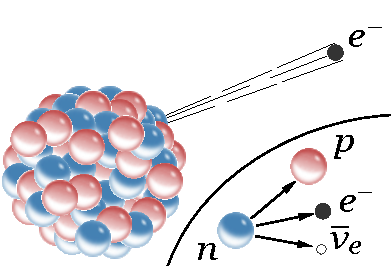
\includegraphics[width=\columnwidth]{../figures/Beta-minus_Decay.pdf}
		\tiny \url{https://en.wikipedia.org/wiki/Beta_decay}
			
	
	\end{columns}
\end{frame}

\begin{frame}{\be-henfald}
	Tilladte overgange:
	\begin{equation*}
	\onslide<2->{\Delta J = 0, \pm1,\ \Delta T = 0, \pm 1,\ \text{og}\ \Delta \pi = 0}
	\end{equation*}
	\onslide<3->{Spin, paritiet og isospin: $J^\pi ; T$}
	\onslide<4->{
		\begin{figure}
			\centering
			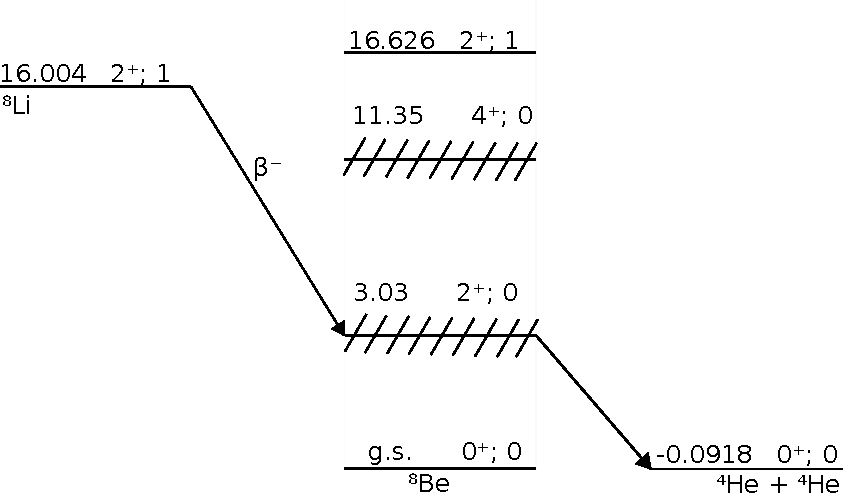
\includegraphics[width=.6\columnwidth]{../figures/DecayScheme.pdf}
		\end{figure}
	}
\end{frame}

\begin{frame}{\al-henfald}
	\begin{columns}
		\column[]{0.6\textwidth}
		Udsendelsen af \al-partikel\\
		\onslide<1->{Q-værdi:
			\begin{equation*}
			Q_\alpha = \left[ m\left(^A_Z X\right) - m\left( ^{A-4}_{Z-2} X' \right) -m_\alpha \right]c^2
			\end{equation*}
		}
		\column[]{.4\textwidth}
		\onslide<1->\includegraphics[width=\columnwidth]{../../Pictures/aal.png}
		\tiny \url{https://en.wikipedia.org/wiki/Alpha_decay}
	\end{columns}

\end{frame}